\begin{figure}[H]
    \centering
    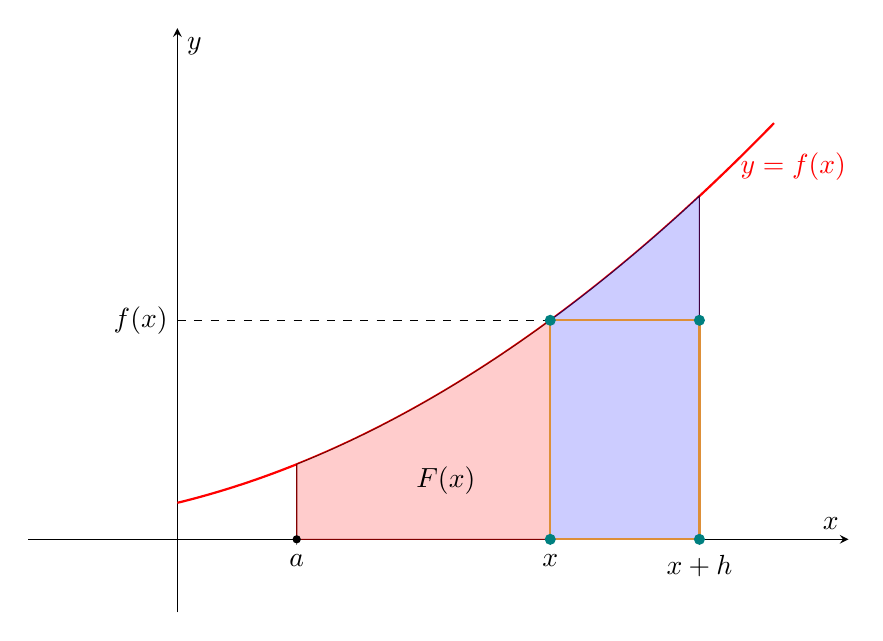
\begin{tikzpicture}
        \begin{axis}[
            axis lines=middle,
            xlabel=$x$,
            ylabel=$y$,
            xtick={0.8, 2.5, 3.5},
            xticklabels={$a$, $x$, $x+h$},
            ytick=\empty,
            xmin=-1, xmax=4.5,
            ymin=-1, ymax=7,
            width=12cm,
            height=9cm,
            clip=false,
            % Khai báo hàm f(x) để vẽ
            declare function={
                myfunc(\t) = 0.2*\t^2 + 0.5*\t + 0.5;
            }
        ]
        
        % Tọa độ các điểm chính
        \coordinate (a) at (axis cs:0.8,0);
        \coordinate (x) at (axis cs:2.5,0);
        \coordinate (x_h) at (axis cs:3.5,0);
        \coordinate (f_x) at (axis cs:2.5, {myfunc(2.5)});
        \coordinate (f_x_h) at (axis cs:3.5, {myfunc(3.5)});
        
        % 1. Vẽ đồ thị hàm số y=f(x)
        \addplot[
            domain=0:4, 
            samples=100, 
            color=red, 
            thick
        ] {myfunc(x)} node[pos=0.9, right] {$y=f(x)$};
        
        % 2. Tô màu vùng F(x) (màu đỏ nhạt)
        \addplot[
            fill=red!20,
            draw=black!50!red,
            domain=0.8:2.5,
        ] {myfunc(x)} \closedcycle;
        \node at (axis cs:1.8, 0.8) {$F(x)$};
        
        % 3. Tô màu vùng F(x+h) - F(x) (màu xanh lá nhạt)
        \addplot[
            fill=blue!20,
            draw=black!50!violet,
            domain=2.5:3.5,
        ] {myfunc(x)} \closedcycle;

        % 4. Vẽ hình chữ nhật màu vàng bên trong vùng màu xanh
        \draw[thick, draw=yellow!50!purple] (axis cs:2.5,0) rectangle (axis cs:3.5, {myfunc(2.5)});

        % 5. Vẽ các đường gióng và nhãn
        % Đường gióng từ x tới f(x)
        \draw[dashed] (axis cs:0, {myfunc(2.5)}) node[left] {$f(x)$} -- (f_x);
        
        % Các điểm chấm trên đồ thị
        \fill[teal] (f_x) circle (2pt);
        % \fill[blue] (f_x_h) circle (2pt);
        \fill[teal] (axis cs:3.5, {myfunc(2.5)}) circle (2pt);
        
        % Các điểm chấm trên trục hoành
        \fill[teal] (x) circle (2pt);
        \fill[teal] (x_h) circle (2pt);
        \fill (a) circle (1.5pt);

        \end{axis}
    \end{tikzpicture}
    \caption{\centering Xấp xỉ tuyến tính của sự gia tăng diện tích. Diện tích của dải hẹp $\Delta F = F(x+h) - F(x)$ có giá trị gần bằng diện tích hình chữ nhật đáy $h$ và chiều cao $f(x)$.}
    \label{fig:fundamental-theorem-1}
\end{figure}